\section{System overview\label{overview}}

A broad overview of the \nr{} backend is provided in Figure
\ref{overview-fig}.  The connecting arrows between different components
usually denote some form of inter-process communication (IPC).  In the
case of \nr{}, this communication is carried out most of the time via
Redis queues and another feature within Redis named pubsub.  Pubsub
is not fault-tolerant, so wherever it's used, the process on
the receiving end also relies on timed polling of some queue holding
output from another module.  The modules are small services that
generally read some information, and then pass derived information to
other services.  Message queues are used extensively
throughout the system, but only the most important queue is represented
in Figure \ref{overview-fig} (the insert queue).  Most services
communicate with the database in some way, but this fact isn't
presented in the diagram.
The most important services
are outlined in greater detail in their own sections
(e.g. Sections \ref{crawling}, \ref{compress}, \ref{ml}), but some
of the smaller services are briefly described next.

\begin{figure}
    \centering
    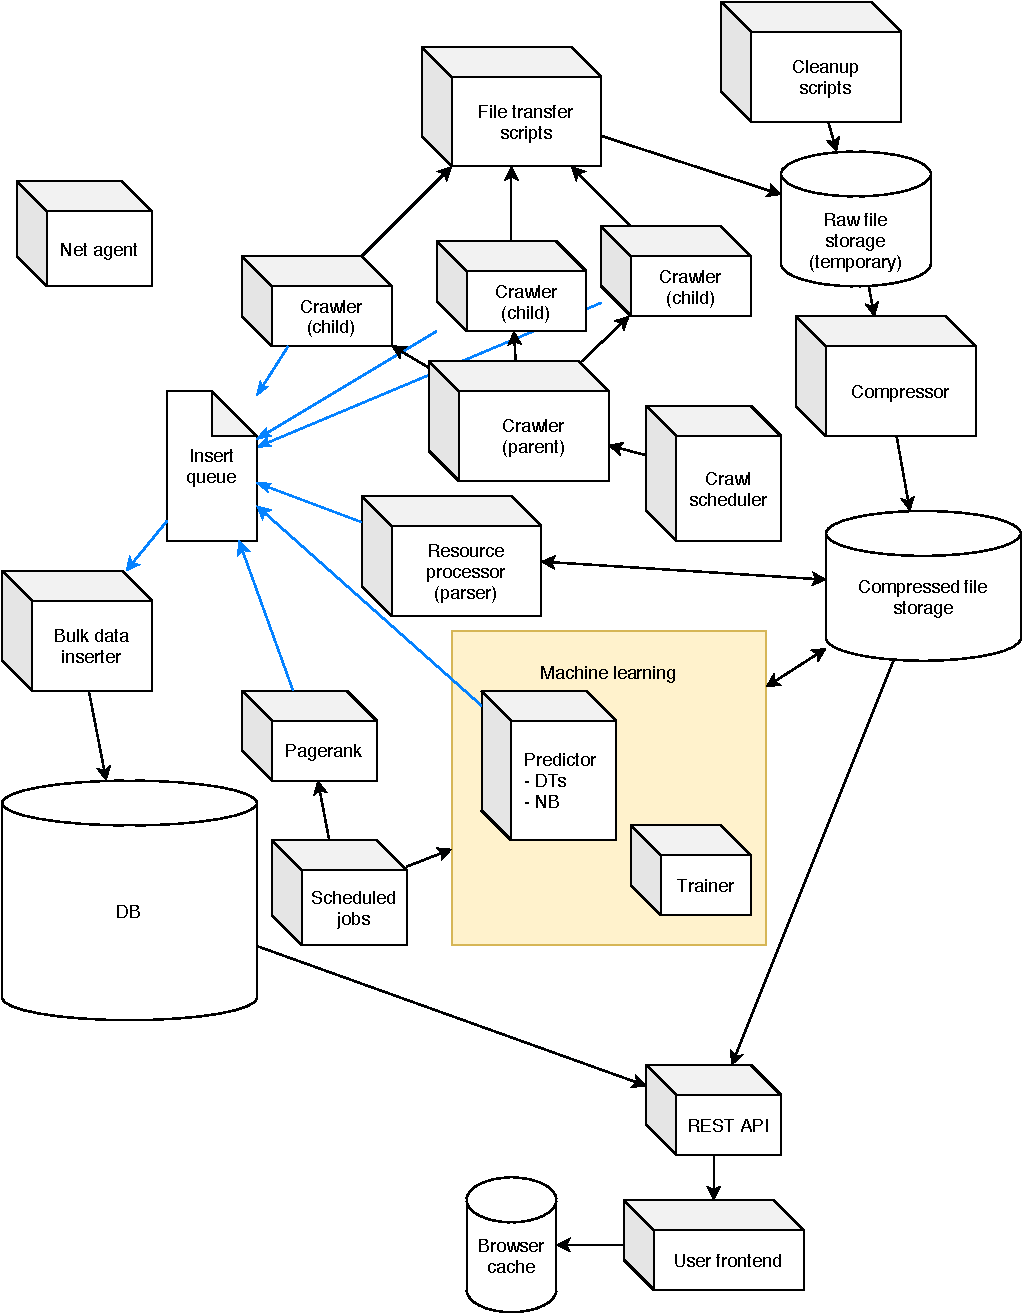
\includegraphics[width=0.95\textwidth]{media/system}
    \caption{
        Broad overview of the system's
        architecture.\label{overview-fig}
    }
\end{figure}

\subsection{The inserter service}
In order to crawl and process large amounts of news data, a strategy
for inserting large amounts of data into a database was needed.

In the \nr{} system, rather than inserting rows into a database one
at a time,
in most cases, rows are appended to a Redis queue.  This queue is
polled at an interval of 400ms, and bulk insert jobs are
created. Experiments were set up to compare the performance
of a large SQL {\tt INSERT} statement with that of a batch CSV
import.  The latter was faster, so the completed inserter service
actually writes data to CSV files, and uses MySQL
{\tt LOAD} statements (every 400ms) to place data into relevant
tables.  This may not be wise when storing critical and inter-connected
personal data, but for large amounts of corpus data, the
few resulting inconsistencies are negligible.
The following parameters were placed in a MySQL server configuration
file in order to speed up the DB server\footnote{Parameters obtained
from various answers on \url{https://stackoverflow.com}}:
\begin{verbatim}
[mysqld]
local-infile = 1 
innodb_doublewrite = 0
innodb_buffer_pool_size = 20G
innodb_log_file_size = 1G
innodb_flush_log_at_trx_commit = 0
\end{verbatim}
\subsection{Hashing\label{hashing}}
Words, URLs and every other {\it entity} stored
in \nr{} databases, is identified by an ID, in the
form of a fixed length cryptographic hash of the entity's
content.  Before hashing, the content is prefixed by the the
entity's own type name.

For example, the URL \url{https://example.com/} would be
identified by the hash of {\tt url:https://example.com/}.
The resulting ID is the first 12 bytes of the cleartext's
{\tt SHA-3} hash.  This hashing schema was chosen in order
to fulfil several requirements:
\begin{enumerate}
    \item The ability to deduce the ID of an entity without
          interacting with the database.\label{pre}
    \item Uniqueness of IDs across the entire
          database (over per-table uniqueness).\label{uniq}
    \item An infeasible hash collision rate among entities.\label{low}
\end{enumerate}
Requirement \ref{pre} ensures that small programs 
can reason about data in the \nr{} system,
without necessarily needing a database connection in order to
obtain the ID of a word, URL, or of anything else.
Knowing the ID of an entity before storing it is also
valuable in terms of concurrency and performance.  If a system
with a large amount of data were to rely on the auto-increment
feature (a popular `ID generator' in MySQL), then
huge amounts of communication to and from the database
would be needed in order for various machines to collaborate.

For example, in the tokenisation stage outlined in Section
\ref{clean}, several processes or machines are tokenising web
resources in parallel.  Most of the documents processed will
contain the word `{\it the}' at least once.  Relying on
auto-increment would lead each machine to send the following
SQL query to the database server:
`{\tt SELECT ID FROM Word WHERE value = "the";}'.
This costly ID check would need to be
carried out for each word in the lexicon of documents being
processed during a given period.  Knowing with certainty that
the ID of `the' is {\tt A91A5E09C79E0221159C8DFF}, without
needing a database connection, is a highly valuable part of a
competitive IR service.

The choice of 12 bytes for the ID can be explained by
considering the birthday paradox and the pigeonhole principle.
If an IR service may potentially store billions of unique objects,
then the ID space needs to be in the region of trillions, to avoid
ID collisions (when the same ID is assigned to two
different objects).  This problem is illustrated in Figure \ref{bday}.
Using 12 byte IDs across different SQL tables renders a collision
practically impossible.

\begin{figure}
    \centering
    \singlespacing
    \begin{tabular}{|l|l|}
    \hline
    Entities & Probability of collision\\
    \hline
    4,194,304               &   0.00000000000001\%\\
    8,388,608               &   0.00000000000004\%\\
    16,777,216              &   0.00000000000017\%\\
    33,554,432              &   0.00000000000071\%\\
    67,108,864              &   0.00000000000284\%\\
    134,217,728             &   0.00000000001136\%\\
    268,435,456             &   0.00000000004547\%\\
    536,870,912             &   0.00000000018189\%\\
    1,073,741,824           &   0.00000000072759\%\\
    2,147,483,648           &   0.00000000291038\%\\
    4,294,967,296           &   0.00000001164153\%\\
    8,589,934,592           &   0.00000004656612\%\\
    17,179,869,184          &   0.00000018626451\%\\
    34,359,738,368          &   0.00000074505805\%\\
    68,719,476,736          &   0.00000298023219\%\\
    137,438,953,472         &   0.00001192092824\%\\
    274,877,906,944         &   0.00004768370445\%\\
    549,755,813,888         &   0.00019073468138\%\\
    1,099,511,627,776       &   0.00076293654275\%\\
    2,199,023,255,552       &   0.00305171124684\%\\
    4,398,046,511,104       &   0.01220628622226\%\\
    8,796,093,022,208       &   0.04881620601105\%\\
    17,592,186,044,416      &   0.19512188925244\%\\
    35,184,372,088,832      &   0.77820617397564\%\\
    70,368,744,177,664      &   3.07667655236558\%\\
    140,737,488,355,328     &  11.75030974154045\%\\
    281,474,976,710,656     &  39.34693402873665\%\\
    562,949,953,421,312     &  86.46647167633872\%\\
    1,125,899,906,842,624   &  99.96645373720974\%\\
    2,251,799,813,685,248   &  99.99999999999873\%\\
    4,503,599,627,370,496   & 100.00000000000000\%\\
    \hline
    \end{tabular}
    \doublespacing
    \caption{The probability of a hash collision when the number of entities reaches different stages, given 12 byte hash IDs.}
    \label{bday}
\end{figure}

Unfortunately, MySQL doesn't have a native 12 byte number type, so the
ID column on each table in this project uses the type {\tt DEC(30)},
which is not as performant as an 8 byte {\tt BIGINT}, and lacks certain
functionality, such as bitwise operations.  Another frustration is that
{\tt DEC(30)} usually maps to a string instead of a big integer in
various programming environments.  For this reason, in hindsight, and
in future projects, {\tt BIGINT} is recommended.

Using the hashing method outlined here with 8 bytes instead of 12,
the probability of a hash collision over a database of 4,294,967,296
identifiable entities is roughly 39\%.  In any case, a few hash
collisions is arguably acceptable in the area of news aggregation
(as opposed to, say, the area of banking).

\subsection{Parsing and processing\label{parse}}

After crawling various websites, {\tt HTML} and headers are stored
locally in files.  But various other formats need to be derived from
these two, in order to compare different machine learning language
models, and choose the best model per task.  Figure \ref{formats}
illustrates these different formats.  The storage strategy for these
different formats is outlined in Section \ref{compress}, and the
motivation for different formats is explained in more detail
in Section \ref{repr}.

To parse {\tt HTML}, the {\tt JSDOM} library was used \cite{jsdom}.
This library was chosen because of its similarity to the
browser's builtin DOM manipulation and tree traversal functions.
Special care was taken by the developer of the library to ensure
backend developers could write code as though they are interacting
with a real browser DOM, rarely with any difference.
This allowed some code to be reused both
for backend (server) and frontend (browser) programs.  For example,
in a later section, AdaBoost decision tree models
are applied to documents via the user's browser.  The model is
stored within the browser's cache.  More information about this
process is provided in Section \ref{privacy}.

\begin{figure}
    \centering
    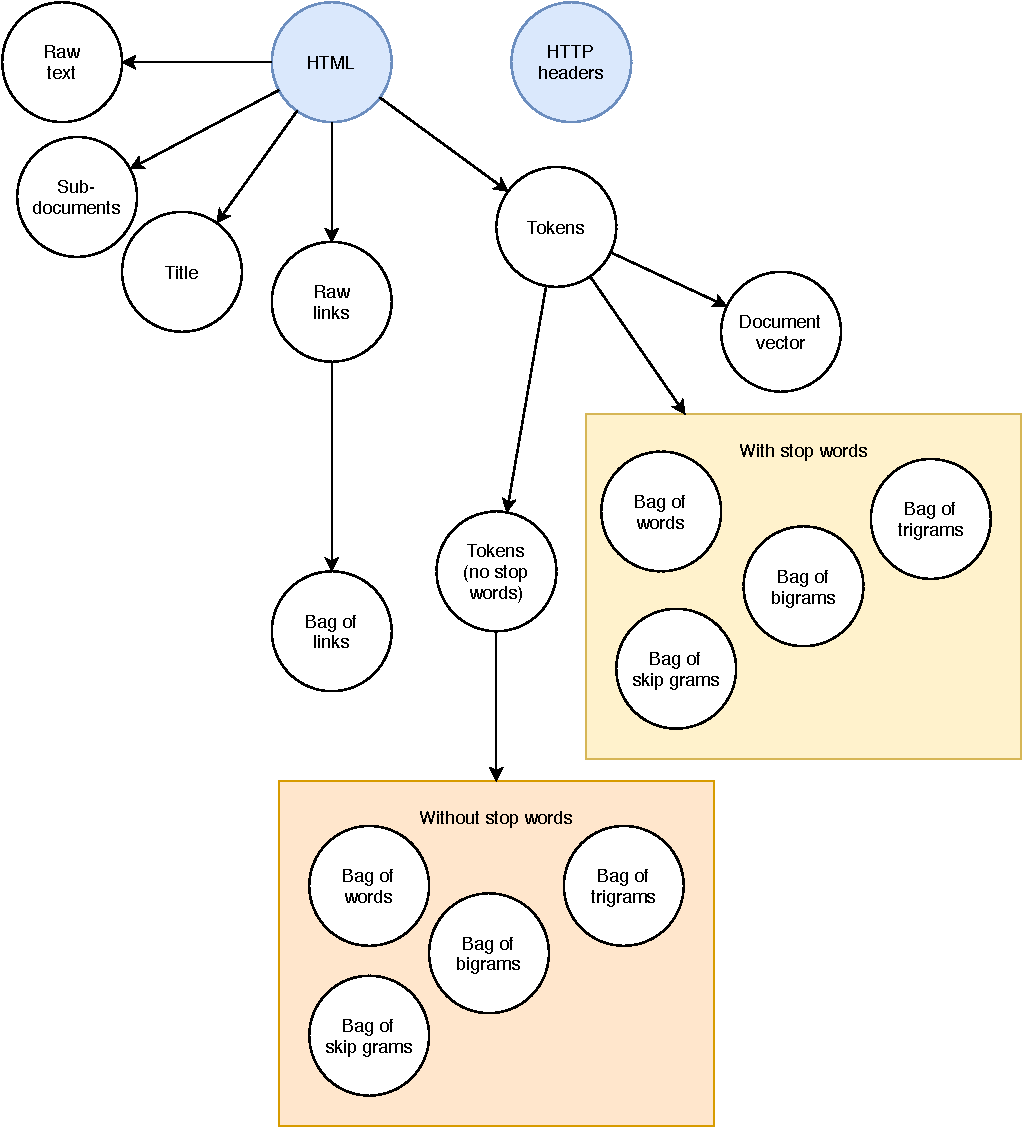
\includegraphics[width=\textwidth]{media/formats}
    \caption{
        The process by which different experimental
        resource models are created.  Blue nodes are models 
        created by the crawler.  The others are
        created later. A comparison of these models, and their
        relative performance in text classification, is
        provided in Section \ref{model-results}.\label{formats}
    }
\end{figure}

\subsection{Net agent}

A {\it net agent} program runs on each machine in the \nr{}'s
network of machines.  The program has two varieties, one for
the parent node (where files and the database are located),
and another for child nodes.  The program is used for
system motitoring, propagating settings from the parent
node, and other {\it housekeeping} tasks.